\section{Transcodificação Rápida para o AV1}
\label{cap:7.4}

Nesta seção, apresentamos as modificações realizadas nos diversos decodificadores e no codificador de referência do AV1 para permitir o desenvolvimento da transcodificação rápida proposta neste capítulo, indicando pontos que são compartilhados em diversas fases de execução do \textit{pipeline} proposto. Para possibilitar uma apresentação mais clara, o conteúdo encontra-se dividido em dois pontos: proposta de algoritmo de transcodificação rápida (subseção \ref{cap:7.4.1}) e modificações necessárias para adequar os decodificadores ao algoritmo desenvolvido de transcodificação rápida (subseção \ref{cap:7.4.2}).

\subsection{Proposta de Algoritmo de Transcodificação Rápida}
\label{cap:7.4.1}

Antes de apresentar a nossa proposta, se faz necessário compreender o fluxo de execução do algoritmo de particionamento de blocos do software de referência do AV1, em sua versão 3.5.0, representado na Figura \ref{fig:30}. Nesta figura, observam-se quatro conjuntos principais de processos: 

\begin{itemize}
    \item \textbf{Blocos verdes}, indicando de início e fim de processos;

    \item \textbf{Blocos cinzas}, indicando processos de predição intraquadro ou interquadros nos blocos daquele tipo de particionamento;

    \item \textbf{Blocos azuis}, indicando processos de podas antecipadas realizadas através de modelos preditivos nativos do \textit{libaom};

    \item \textbf{Bloco branco}, indicando um condicional que avalia se as podas realizadas não geraram situação impossível, por exemplo, uma repetição infinita ou uma impossibilidade de obter melhores resultados de custo taxa-distorção (rd-cost).
\end{itemize}

\begin{figure}
    \centering
    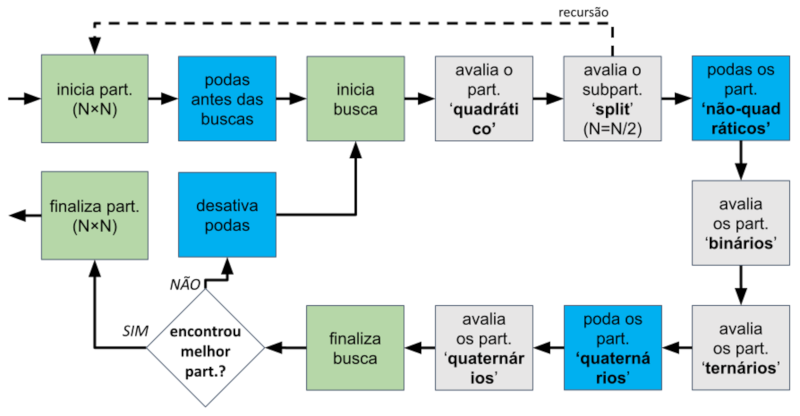
\includegraphics[width=0.75\textwidth]{FIGURES/fig_30.png}
    \caption{Diagrama de execução da busca da melhor estrutura de particionamentos no \textit{libaom} 3.5.0. Fonte: Elaborada pelo autor.}
    \label{fig:30}
\end{figure}

Há uma recursão explícita no fluxo de particionamento de blocos do AV1, conforme pode ser observado na Figura \ref{fig:30}. Recursão essa que é aplicada para quatro novos processos, cada um relacionado a um novo ramo da árvore de particionamentos. Nas versões anteriores do \textit{libaom}, era obrigatório o teste de predição intraquadro ou interquadros no bloco em processamento com ao menos um modo de predição, o que explica a obrigatoriedade da predição simples aplicada ao nosso trabalho de H.265/HEVC-para-AV1 na seção \ref{cap:6.1}. Contudo, na versão atual do \textit{libaom}, é possível ignorar a predição, caso o processo de podas realizado antes das buscas assim identifique. Neste caso, apenas o modo de particionamento \textit{SPLIT} é executado, ou seja, a recursão é aplicada.

Como já foi esclarecido, os modelos preditivos gerados na proposta de transcodificador rápido decidem sobre o particionamento ou não do bloco atual. Logo, modificamos o fluxo de execução do particionamento de blocos da Figura \ref{fig:30} para incluir os processos de antecipação do modo \textit{SPLIT}, realizado através dos modelos preditivos propostos neste capítulo, conforme pode ser visto em laranja na Figura \ref{fig:31}.

\begin{figure}
    \centering
    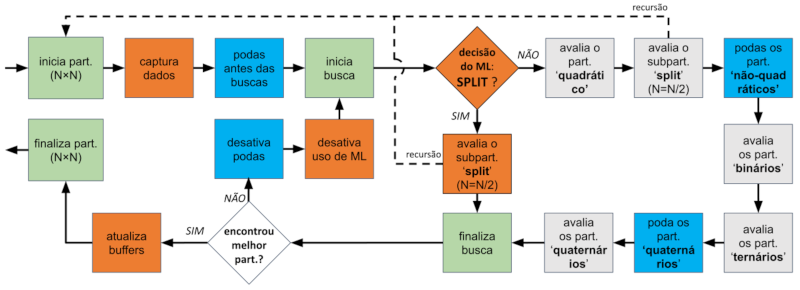
\includegraphics[width=\textwidth]{FIGURES/fig_31.png}
    \caption{Diagrama de execução da busca da melhor estrutura de particionamentos no transcodificador rápido (\textit{libaom} 3.5.0). Fonte: Elaborada pelo autor.}
    \label{fig:31}
\end{figure}

Na Figura \ref{fig:31} observam-se cinco modificações (destacados em laranja), cada uma responsável por um processo específico, conforme descrevemos abaixo:

\begin{enumerate}[1.]
    \item Selecionar informações nos \textit{buffers} que alimentam o modelo preditivo;

    \item Avaliar respostas dos modelos preditivos propostos;

    \item Utilizar o tipo de particionamento \textit{SPLIT}, caso os modelos propostos assim indiquem;

    \item Desativar o modelo de aprendizado de máquina proposto, caso o condicional do fluxo principal de execução do particionamento de blocos do \textit{libaom} assim o indique;

    \item Atualizar informações processadas aos \textit{buffers} que alimentam o modelo preditivo proposto.
\end{enumerate}

Dentre esses cinco processos implementados no fluxo de execução do particionamento de blocos, destacam-se dois: atualização de \textit{buffers} e captura de dados. O primeiro destes processos tem como objetivo ler as informações extraídas tanto do decodificador como do codificador e armazená-las em estruturas de dados que, durante o segundo destes processos, alimentará os modelos preditivos. É após a resposta positiva do condicional do fluxo de execução do particionamento de blocos que se torna possível a obtenção das decisões obtidas naquele nível de profundidade do AV1. Logo, a atualização das estruturas de dados que alimentam o modelo preditivo só ocorre neste momento, independente da profundidade processada. Os tipos de dados extraídos, tanto do decodificador como do codificador, são idênticos, pois dessa forma se reduz significativamente a complexidade de adaptação de estruturas de dados e modificações de tipos de dados ao adaptar o algoritmo de transcodificador rápido para outros formatos. Portanto, as seguintes variáveis são coletadas:

\begin{enumerate}[1.]
    \item \textbf{Nível de Profundidade}: indica quantas vezes a árvore de particionamento se dividiu. Essa variável está diretamente ligada ao rótulo a ser predito. Esperam-se valores inteiros e maiores que 0, onde 0 indica que o superbloco não se subdividiu (ou seja, um bloco quadrático equivalente a 128$\times$128). O valor máximo esperado é 5, onde a árvore atingiu a profundidade máxima, ou seja, bloco de tamanho 4$\times$4. Ressalta-se que atribuímos 0 para blocos 128$\times$128, pois este é o maior tamanho de bloco atualmente disponível nos formatos de codificação de vídeo;

    \item \textbf{Tamanho de bloco}: informa um código referente ao tamanho de bloco utilizado. É relevante utilizar essa variável em conjunto com a anterior porque, apesar de ser possível inferir a profundidade da árvore por meio do tamanho de bloco, o inverso não é verdade. Por exemplo, o bloco 32$\times$32 em essência está na profundidade 2, mas caso o AV1 utilize algum tipo de particionamento ternário (tipo \textit{AB}), esse mesmo tamanho de bloco estará, na verdade, na profundidade 1. São esperados valores inteiros, correspondentes à identificação interna do software do codificador para esses tamanhos de blocos;

    \item \textbf{Orientação dos blocos}: informa qual é a orientação dos blocos não quadráticos utilizados naquela profundidade. Essa variável complementa as duas variáveis anteriores, pois auxilia a identificar o tamanho do bloco com a profundidade. São esperados valores inteiros, onde 0 indica o uso de blocos quadráticos, código 1 indica orientação horizontal e código 2 indica orientação vertical; 

    \item \textbf{Modo de predição}: informa o código do modo de predição intraquadro ou interquadros utilizado pelo codificador;

    \item \textbf{Tipo de predição}: complementa a variável anterior, indicando qual foi o tipo de predição realizado, se intraquadro (código 0) ou interquadros (código 1). Essa variável é utilizada porque há uma tendência de blocos menores serem codificados com predição do tipo intraquadro, o que pode auxiliar o modelo a identificar possíveis subparticionamentos de blocos.
\end{enumerate}

No algoritmo de transcodificação rápido desenvolvido, sumarizado na Figura \ref{fig:31}, as informações que alimentam os modelos preditivos são capturadas e armazenadas em \textit{buffers}, que contêm todas as variáveis acima citadas de regiões vizinhas ao bloco em processamento (B.P.). A escolha por regiões vizinhas como fonte de informações para uso em modelos preditivos já foi observada em \citet{bib:guo_2018}, indicando que é particularmente mais eficiente em vídeos de resolução HD1080 ou superior. Desta forma, representamos na Figura \ref{fig:32} as regiões nas quais as variáveis acima citadas serão capturadas, a fim de alimentar o modelo preditivo. Nesta figura, observam-se cinco regiões (A, B, C, D e E) distantes N pixels da posição do B.P., nas quais serão capturados cinco valores de cada uma. Logo, os modelos preditivos utilizados nas soluções propostas neste capítulo utilizam 25 atributos para embasar as suas decisões. Observe que, por utilizarmos regiões vizinhas ao B.P., as regiões B, C, D e E, eventualmente, podem estar localizadas aquém dos limites do quadro, isto é, suas posições x e y podem ser menores que zero. Nesses casos excepcionais, os modelos preditivos estarão desabilitados para uso naquela iteração da busca da melhor estrutura de particionamentos no \textit{libaom}.

\begin{figure}
    \centering
    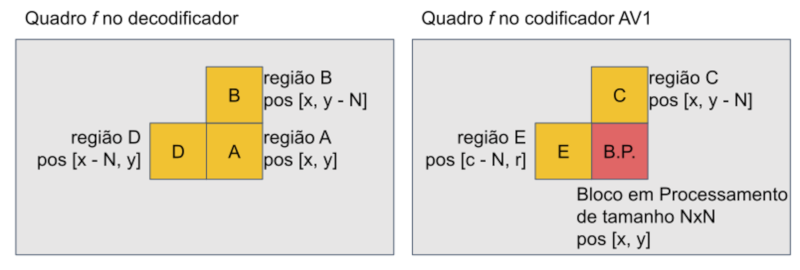
\includegraphics[width=0.75\textwidth]{FIGURES/fig_32.png}
    \caption{Representação em alto nível das regiões onde atributos são selecionados para alimentar o modelo preditivo. Fonte: Elaborada pelo autor.}
    \label{fig:32}
\end{figure}

Sete matrizes compõem as estruturas de dados utilizadas para armazenar as informações, sendo quatro dedicadas ao armazenamento das informações provenientes do decodificador, quatro para armazenar as decisões do codificador e uma matriz auxiliar (AUX) utilizada para preenchimento das seis matrizes anteriores. É nesta matriz AUX que serão armazenadas todas as informações observadas durante a decodificação e a re-codificação, em áreas de 4$\times$4 pixels e, desta forma, utilizadas para alimentar corretamente as outras matrizes. Cada uma das matrizes principais são utilizadas para o armazenamento de informações relativas ao nível de profundidade ao qual estão associadas. Conforme pode ser visto na Figura \ref{fig:33}, cada uma das matrizes principais possui um tamanho distinto e proporcional à resolução do vídeo, onde cada ponto (P) dessa matriz representa uma área de igual tamanho de bloco ao qual está sendo processado (128$\times$128, 64$\times$64 ou 32$\times$32). Assim, considerando um vídeo de resolução HD1080, a matriz com P igual a 128$\times$128 terá o tamanho de 15$\times$9. Ao final do processo ``\textit{Atualiza Buffers}'', apresentado na Figura \ref{fig:32}, a matriz auxiliar é utilizada para geração de médias que preencherão as matrizes principais.

\begin{figure}
    \centering
    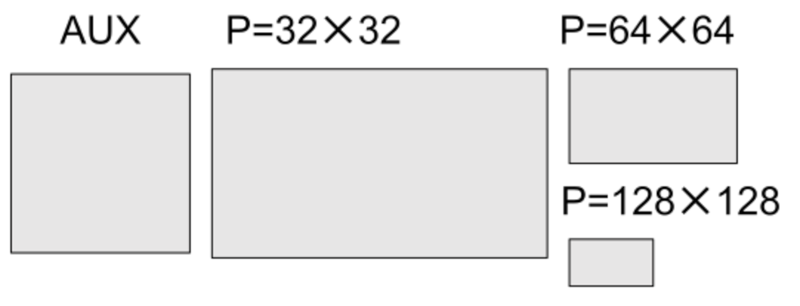
\includegraphics[width=0.5\textwidth]{FIGURES/fig_33.png}
    \caption{Representação do tamanho das matrizes utilizadas pelas estruturas de dados implementadas. Fonte: Elaborada pelo autor.}
    \label{fig:33}
\end{figure}

\subsection{Informações Extraídas dos Softwares Decodificadores}
\label{cap:7.4.2}

Na subseção anterior apresentamos o algoritmo proposto para transcodificação rápida para o formato AV1, cuja estrutura geral pode ser adaptada para demais propostas de transcodificador. Como discutido na subseção anterior, todas as regiões apresentadas na Figura \ref{fig:32} armazenam os mesmos tipos de informações. Logo, cada um dos decodificadores considerados precisam exportar as mesmas informações, na medida que isso seja possível. Nesta subseção, discutimos de que forma isso foi implementado.

Um dos dados exportados não versa sobre nenhuma das cinco variáveis necessárias para preenchimento das matrizes principais, mas identifica a posição do bloco ao qual correspondem as informações no quadro decodificado. Enquanto os padrões H.265/HEVC e H.266/VVC utilizam posições reais de pixels para identificar regiões do quadro, ou seja, um bloco na posição [384, 512] está de fato nesta posição no quadro, no padrão H.264/AVC e nos formatos VP8, VP9 e AV1, cada posição de bloco não é um valor absoluto de pixel, mas um referencial para o menor conjunto de blocos existente naquele formato. Dessa forma, a posição [384, 512] no formato AV1 indica um bloco localizado a partir do pixel [1536, 2048], por exemplo. Portanto, as posições de bloco representadas em cada decodificador precisam ser adequados para o formato utilizado pelo AV1, seguindo as regras abaixo:

\begin{itemize}
    \item Se a posição for originária de um vídeo no formato VP8 ou do padrão H.264/AVC, multiplicar os valores na tupla por quatro;

    \item Se a posição for originária de um vídeo no formato VP9, multiplicar os valores da tupla por dois;

    \item Se a posição for originária de um vídeo codificado nos padrões H.265/HEVC ou H.266/VVC, dividir os valores da tupla por quatro.
\end{itemize}

Já em relação à obtenção das variáveis propriamente ditas, as duas que não precisam ser adaptadas em nenhum dos cinco formatos utilizados na decodificação (VP8, VP9, H.264/AVC, H.265/HEVC e H.266/VVC) são as variáveis ``\textit{Orientação do Bloco}'' e ``\textit{Modo de Predição}''. No caso da primeira, basta observar os tamanhos de blocos utilizados; na segunda, exporta-se a informação sem nenhum de adaptação de valores, já que cada formato de codificação possui uma identificação numérica própria para esses modos de predição. Dessa forma, preferimos manter essa identificação inalterada. A variável ``\textit{Nível de Profundidade}'', como discutido na subseção anterior, contabiliza o número de vezes que o modo \textit{SPLIT} foi escolhido. No entanto, apenas o padrão H.266/VVC possui nível zero, por ser o único formato que oferece tamanho de bloco igual a 128$\times$128, além do AV1. Para todos os demais formatos, adaptou-se a contagem de particionamentos para torná-la equivalente à numeração observada no formato AV1. A única exceção recai para o VP8, que só possui dois tamanhos de blocos: 16$\times$16 e 4$\times$4; logo, há somente dois níveis de profundidades no VP8: 3 e 5.

Ainda no formato VP8, o tamanho de bloco utilizado já indica o tipo de predição realizado, isto é, se intraquadro (blocos 4$\times$4) ou interquadros (blocos 16$\times$16). Por outro lado, apesar dos formatos H.265/HEVC e H.266/VVC compartilharem a variável que indica se o tipo de predição é intraquadro ou interquadros, o tamanho de bloco não é fator decisivo para essa informação. Inclusive, esses dois padrões possuem uma complexa estrutura de particionamentos (como visto no capítulo \ref{cap:2}), havendo uma estrutura composta por sub-estruturas, cada uma com uma finalidade específica para a codificação, vide \citet{bib:h265} e \citet{bib:vvc_partitioningStructure}. Como essas estruturas não são repassadas ao decodificador, não é possível obter diretamente maiores informações sobre elas. No decodificador, podem-se obter apenas informações sobre a largura e a altura dos blocos, o que utilizamos para inferir as variáveis de ``\textit{Tamanho de Bloco}'' e ``\textit{Orientação do Bloco}''.
